\chapter{Desenvolvimento}
Este capítulo terá como foco detalhar o sistema proposto, apresentar sua modelagem e comentar seus aspectos técnicos e funcionais. Serão apresentados os requisitos funcionais e não funcionais, obtidos por meio de análise de requisitos, nos quais a implementação tomou como base, além de mostrar diagramas UML que fundamentam diferentes aspectos do sistema. \cite{Sommerville2011} define o estágio de desenvolvimento sendo composto por todas as atividades envolvidas no desenvolvimento do sistema, como definição de requisitos, projeto de sistemas, engenharia de hardware e software, integração de sistemas e testes.

O \emph{software} implementado se baseou nas principais práticas de engenharia de \emph{software}, tornando o processo de desenvolvimento fluido, adotando o modelo em cascata como metodologia de desenvolvimento.

\section{Descrição geral}
O sistema implementado é uma API REST visando manter um registro de todas as ações tomadas pelo usuário do aplicativo Carteira Digital do Restaurante Universitário da UEA (APP-RU). O sistema é uma solução proposta à problemática de salvar dados de alunos de forma segura, utilizando a Blockchain como meio de persistir informações de forma íntegra e privativa. Com isto, logs do tipo informacional são guardados na rede distribuída. A partir de requisições, a API REST processa o pedido do usuário, captando os dados necessários para realizar um registro da ação executada na plataforma Ethereum. Exemplificando: se um aluno comprar um ticket, uma requisição é disparada, sendo captada pela aplicação Python e extraindo os dados necessários para persistir os dados na Blockchain, por meio da chamada de um contrato inteligente.

\section{Tecnologias utilizadas}
Para desenvolver o projeto, optou-se pela linguagem de programação Python para criar a API REST e a linguagem Solidity para implementar o contrato inteligente que é executado na plataforma Ethereum. 

De modo a facilitar a execução do código produzido e o processo de implantação do sistema, utilizou-se a tecnologia Docker. As tecnologias e dependências utilizadas neste projeto são:

\begin{table}[H]
    \centering
    \begin{tabular}{ | p{3cm} | p{1.75cm} | p{10cm} |}
        \hline
        \textbf{Biblioteca} & \textbf{Versão} & \textbf{Utilidade}\\
        \hline

        Docker & 20.10.16 & Virtualização de imagens  \\
        \hline

        Python & 3.10 & Linguagem de programação para construção da solução. Disponibilizada via imagem Docker  \\
        \hline

        Flask & 2.2.2 & \emph{Microframework} destinado à construção de APIs  \\
        \hline

        flask-smorest & 0.40.0 & Serialização de dados e geração de documentação da API.  \\
        \hline

        python-dotenv & 0.21.0 & Gerenciamento de variáveis de ambiente  \\
        \hline

        Web3.py & 5.31.3 & Conexão com a Blockchain  \\
        \hline

        Solidity & 0.8 & Desenvolvimento de contratos inteligentes  \\
        \hline
    \end{tabular}
    \caption{Tecnologias utilizadas para o desenvolvimento da solução}
    \label{tab:tecnologias_utilizadas}
\end{table}

A \emph{testnet} usada neste trabalho é a rede Goerli (chamada também de Görli), junto da rede Sepolia. Goerli surgiu em 2019 e é uma das principais redes de teste públicas da plataforma Ethereum, juntamente com a \emph{testnet} Sepolia. Diferentemente de outras redes de teste que se tornaram depreciadas como Ropsten e Rinkeby, Goerli é mantida e desenvolvida pela própria comunidade Ethereum. A rede possui um explorador de transações próprio tal como existe com a \emph{mainnet}, chamado de Goerli Etherscan, que fornece uma interface intuitiva para visualizar dados da Blockchain, como transações efetuadas, contratos implantados e informações sobre determinados blocos da rede.

\section{Modelagem do sistema}
\subsection{Requisitos}

\subsubsection{Requisitos funcionais}
\begin{table}[H]
    \centering
    \begin{tabular}{ | p{3cm} | p{10cm} |}
        \hline
        \textbf{Identificador} & \textbf{Descrição}\\
        \hline

        RF01 & A API REST deverá salvar registros (\emph{logs}) de ações executadas pelo usuário no APP-RU na Blockchain  \\
        \hline
        
        RF02 & Os dados devem ser persistidos na Blockchain por meio do uso de um contrato inteligente implantado na plataforma Ethereum \\
        \hline

        RF03 & A API REST deverá ser capaz de retornar dados referentes ao uso do APP-RU \\
        \hline

        RF04 & A persistência de dados deverá ocorrer por meio do uso do formato de dados \emph{string} na Blockchain \\
        \hline

        RF05 & A API REST deverá ser capaz de registrar em sua mensagem de \emph{log} a data e a hora da realização de uma interação com o APP-RU de um determinado usuário \\
        \hline

        RF06 & A API REST deverá ser capaz de registrar em sua mensagem de \emph{log} o módulo requisitado por um determinado usuário \\
        \hline

        RF06 & A API REST deverá ser capaz de registrar em sua mensagem de \emph{log} uma mensagem referente ao ato realizado por um determinado usuário, junto de sua identificação única \\
        \hline

    \end{tabular}
    \caption{Requisitos funcionais}
    \label{tab:my_label}
\end{table}

\subsubsection{Requisitos não funcionais}
\begin{table}[H]
    \centering
    \begin{tabular}{ | p{3cm} | p{10cm} |}
        \hline
        \textbf{Identificador} & \textbf{Descrição}\\
        \hline
        
        RNF01 & A aplicação local deverá ser executada isoladamente em um contêiner Docker, garantindo assim um melhor gerenciamento de dependências e um processo de implantação mais ágil \\
        \hline
        
        RNF02 & A API REST deverá estar documentada por meio do uso do padrão OpenAPI 3.0 \\
        \hline

        RNF03 & O sistema deverá ser utilizado por meio de requisições à API REST, realizando comunicação com seus clientes com o uso do formato de dados JSON \\
        \hline
        
        RNF04 & O sistema deverá, por meio do uso da Blockchain, garantir confiabilidade, integridade, disponibilidade aos dados trafegados \\
        \hline

        RF05 & A comunicação com a Blockchain se dará com o uso da plataforma Ethereum, devendo ser mediada por meio de um provedor Infura, garantindo estabilidade e robustez nas transações
        \\
        \hline

        RNF06 & O sistema deverá ser de fácil manutenção \\
        \hline

        RNF07 & O sistema deverá ser facilmente extensível, possibilitando a implementação de novas funcionalidades em tempo posterior \\
        \hline

        RNF08 & O sistema deverá ser resiliente a falhas de âmbito interno, não admitindo erros capazes de parar o funcionamento da aplicação \\
        \hline
    \end{tabular}
    \caption{Requisitos não funcionais}
    \label{tab:my_label}
\end{table}

\subsection{Diagrama de Casos de Uso}
\begin{figure}
    \centering
    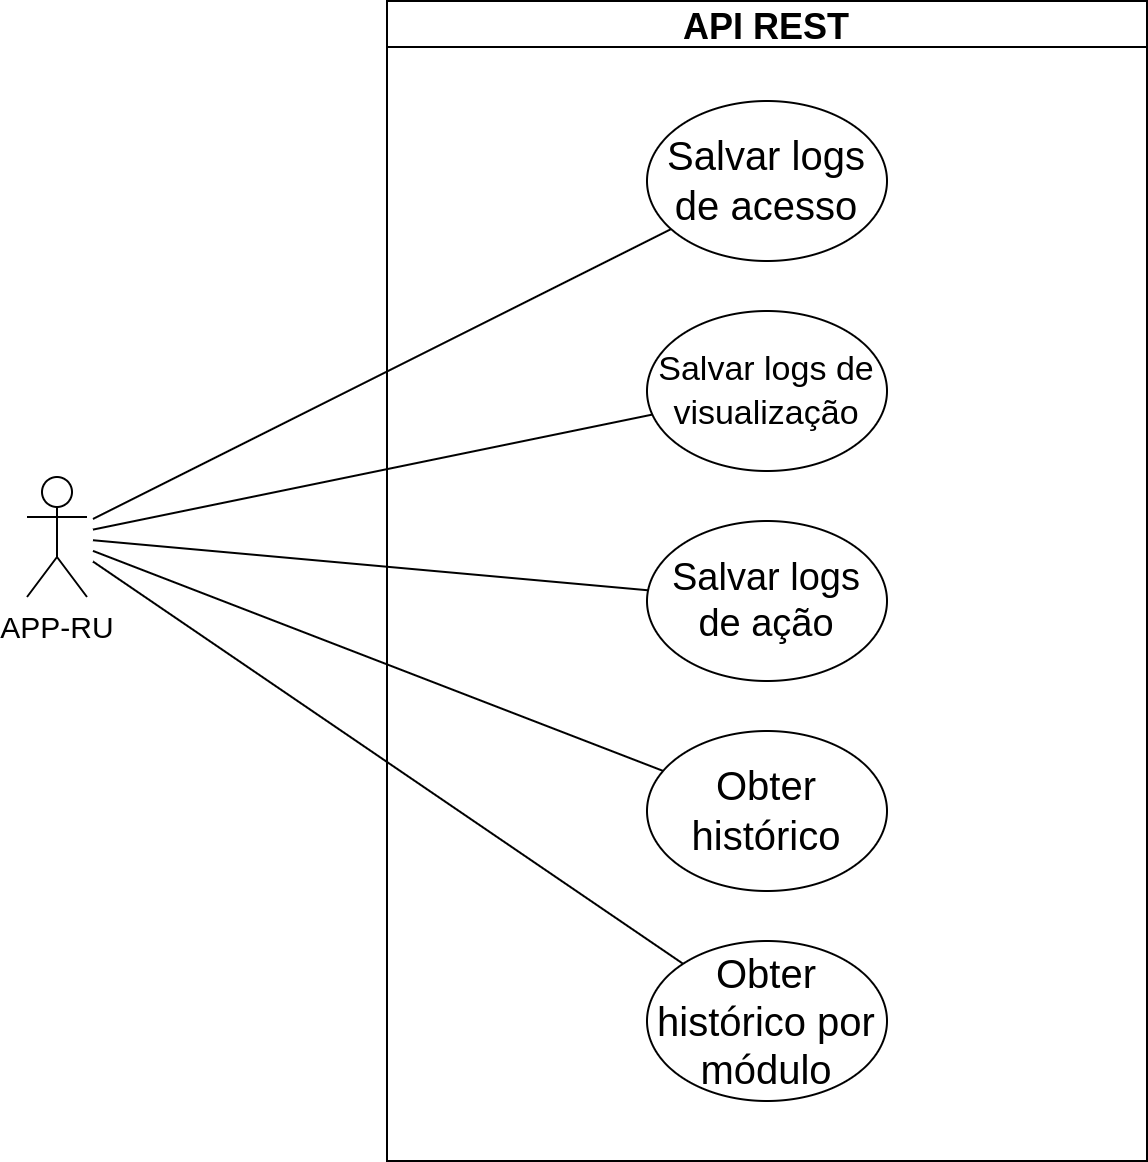
\includegraphics[width=0.75\textwidth]{img/Cap3/diagramas/Diagrama de Casos de Uso.png}
    \caption{Diagrama de Casos de Uso}
    \label{fig:diagrama_casos_uso}
\end{figure}
O papel do Diagrama de Casos de Uso é detalhar quem são os atores, ou seja, as partes envolvidas, e como eles interagem com o sistema. Para \cite{Sommerville2011}, um caso de uso identifica os atores em uma interação e dá nome ao tipo de interação. Os atores podem ser usuários do sistema ou mesmo uma máquina ou um outro sistema.

Neste contexto, um ator é qualquer entidade que faça uso (consuma) da API REST. Em especial, alunos da universidade e administradores do sistema utilizam a API por meio de requisições feitas em seus dispositivos. Outra maneira de de utilizá-la é via uso dos chamados \emph{API Clients}, \emph{softwares} próprios para o envio de requisições que são usados sobretudo em ambientes de desenvolvimento.

O diagrama apresentado na Figura \ref{fig:diagrama_casos_uso} retrata os casos de uso do usuário aluno. Para cada ação realizada pelo aluno, a API disponibiliza um \emph{endpoint} em que são enviados os seus dados. A cada requisição realizada em um \emph{endpoint}, um novo \emph{log} é gerado, sendo posteriormente persistido na plataforma Ethereum.

\newpage
\subsection{Diagrama de Atividades}
\begin{figure}
    \centering
    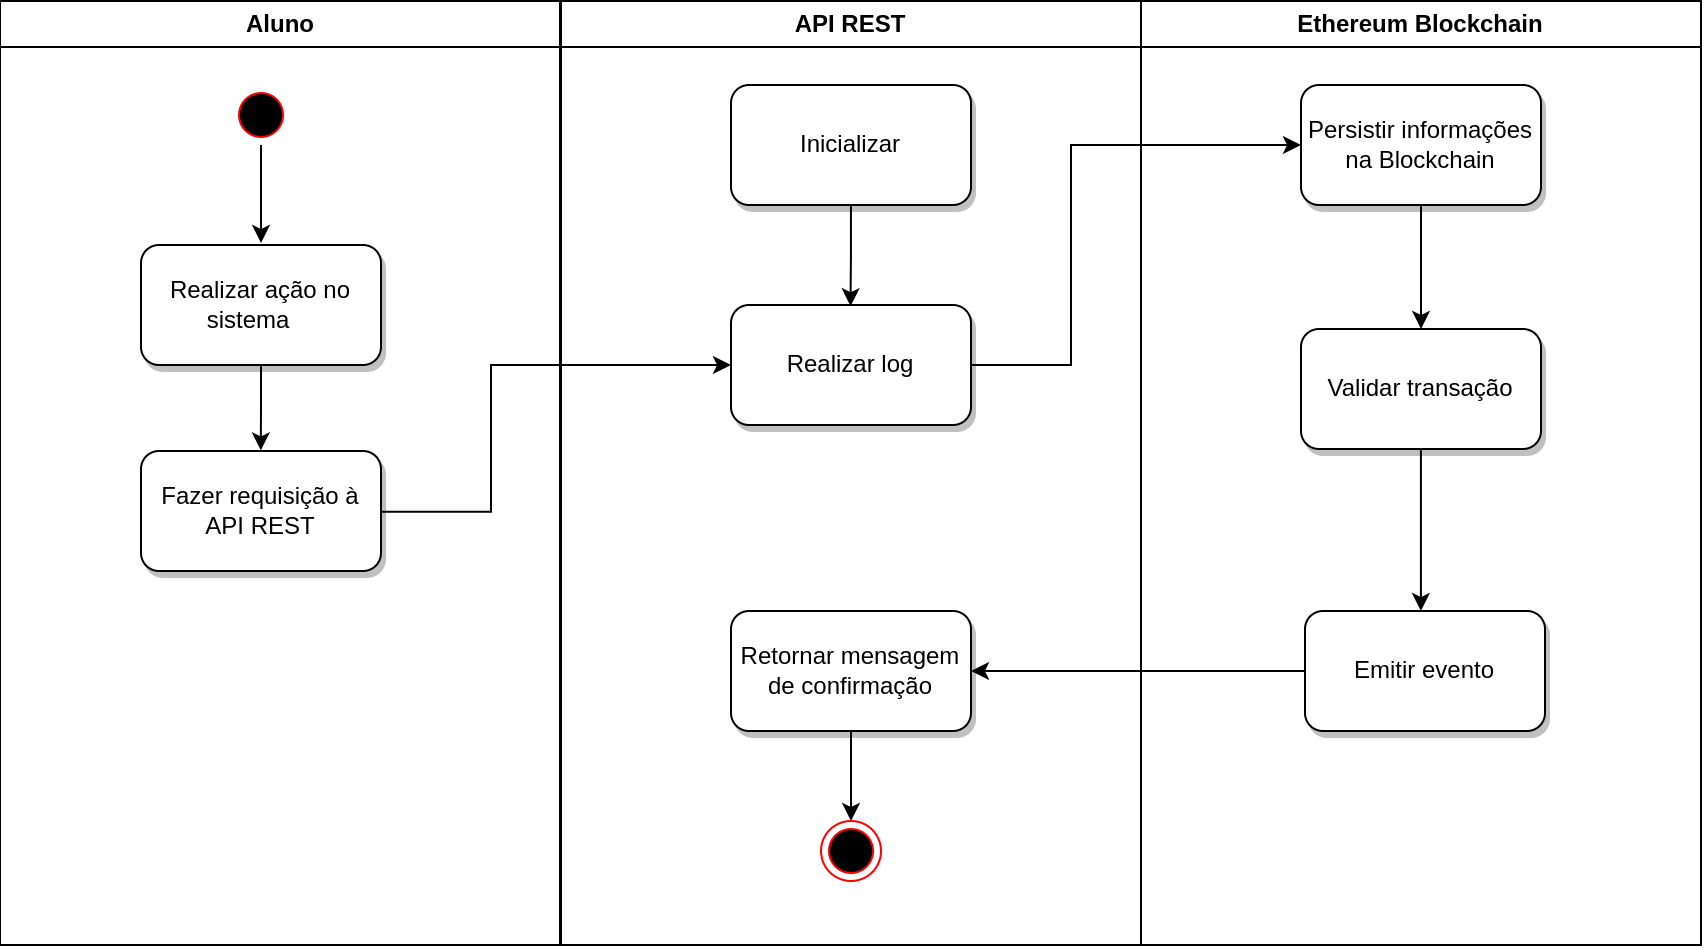
\includegraphics[width=1\textwidth]{img/Cap3/diagramas/Diagrama de Atividade.png}
    \caption{Diagrama de Atividades}
    \label{fig:diagrama_atividades}
\end{figure}
Ao passo em que Diagramas de Casos de Uso detalham o que o sistema deve fazer, os Diagramas de Atividades especificam como o sistema irá alcançar o seu objetivo \cite{Miles2006-fo}. Os Diagramas de Atividades possuem início e fim bem delimitados, representados por círculos preenchidos inseridos no diagrama. Eles exprimem quais são as atividades que compõe um processo dentro do sistema, e o fluxo de controle de uma atividade a outra \cite{Sommerville2011}.

O diagrama aqui apresentado na Figura \ref{fig:diagrama_atividades} ilustra a maneira em que as diferentes partes realizam comunicação para registrar um \emph{log} na plataforma Ethereum. A API REST, após inicializada, recebe uma requisição do usuário e utiliza os dados coletados para realizar uma transação na Blockchain, encarregada de validar esta transação e então emitir um evento à API, concluindo a operação com o envio de uma confirmação ao usuário.

\newpage
\subsection{Diagrama de Sequência}
\begin{figure}
    \centering
    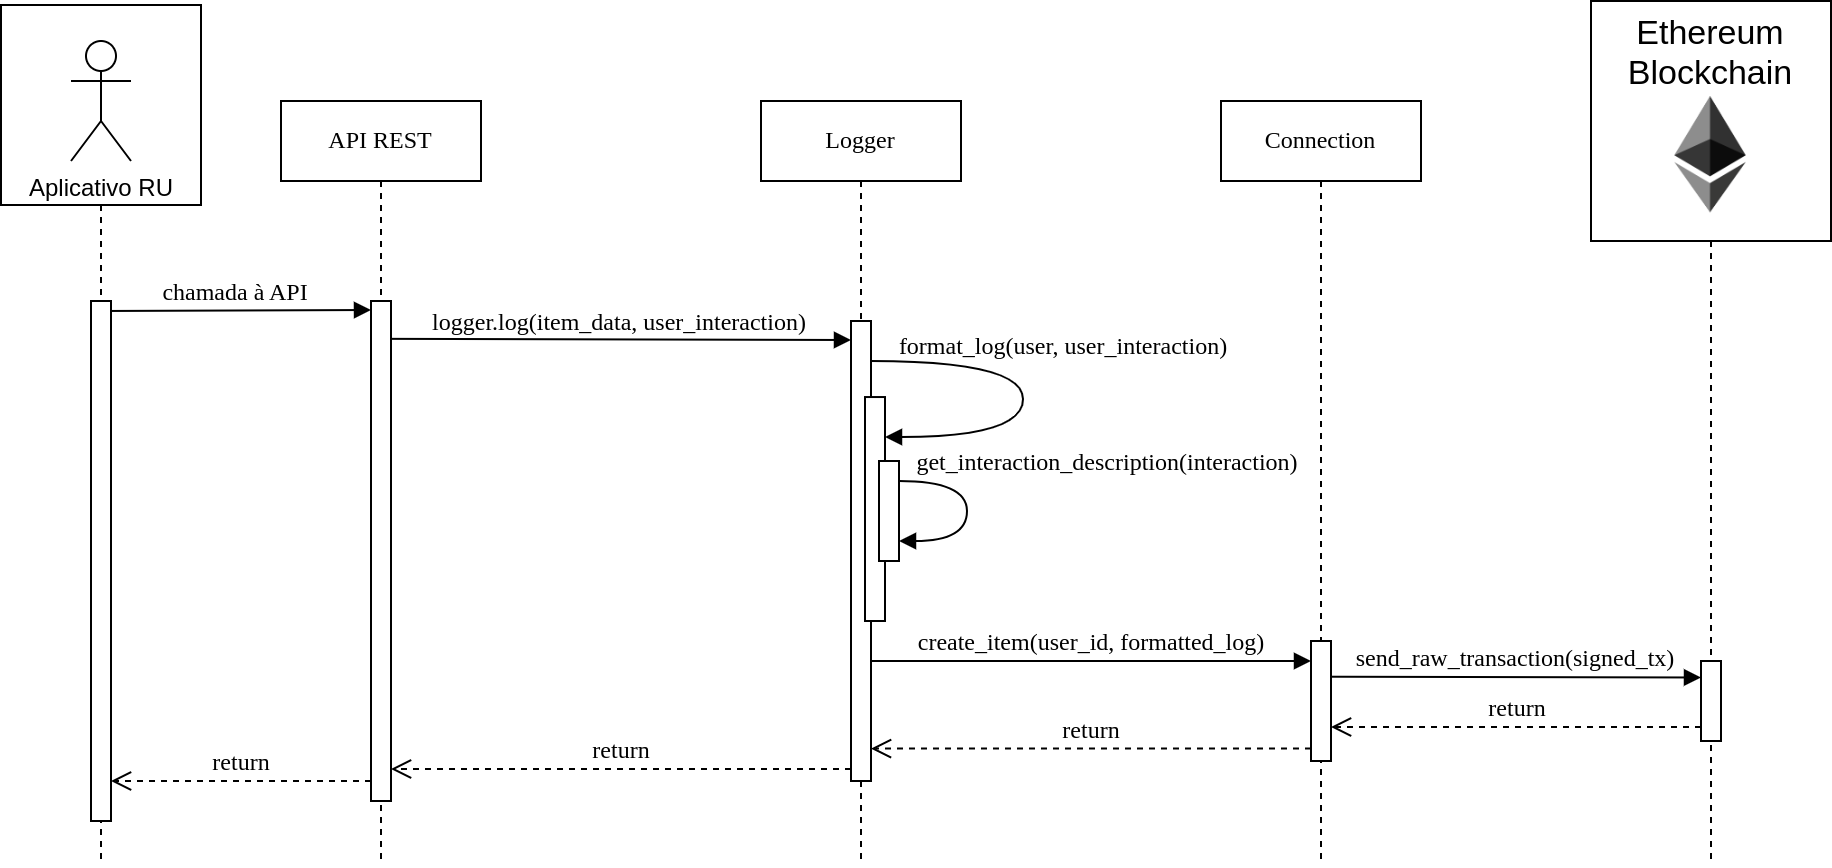
\includegraphics[width=1\textwidth]{img/Cap3/diagramas/Diagrama de Sequência.drawio.png}
    \caption{Diagrama de Sequência da aplicação}
    \label{fig:diagrama_sequencia}
\end{figure}
Com o Diagrama de Sequência conseguimos obter uma visão de como o sistema age para alcançar determinado fim. Nele existem os participantes, as partes do sistema que interagem umas com as outras durante uma sequência \cite{Miles2006-fo}. Dispostos de maneira horizontal entre si, os participantes possuem uma reta vertical em baixo, chamada de linha de vida, ilustrando o seu estado em um determinado instante de tempo.

O diagrama da Figura \ref{fig:diagrama_sequencia} demonstra o encadeamento lógico da troca de mensagens entre os diferentes participantes do sistema, dando ênfase à ordem temporal em que as mensagens foram trocadas. Similar ao Diagrama de Casos de Uso, o Diagrama de Sequência também define atores, entidades que, juntamente com os objetos do sistema, formam os participantes que participam de toda a interação. A mensagem inicial parte do aplicativo Carteira Digital do Restaurante Universitário da UEA, realizando uma chamada à API REST, que então utiliza objetos instanciados do sistema para realizar a lógica de negócio, por fim, culminando na comunicação com a Blockchain Ethereum.

\newpage
\begin{figure}
    \centering
    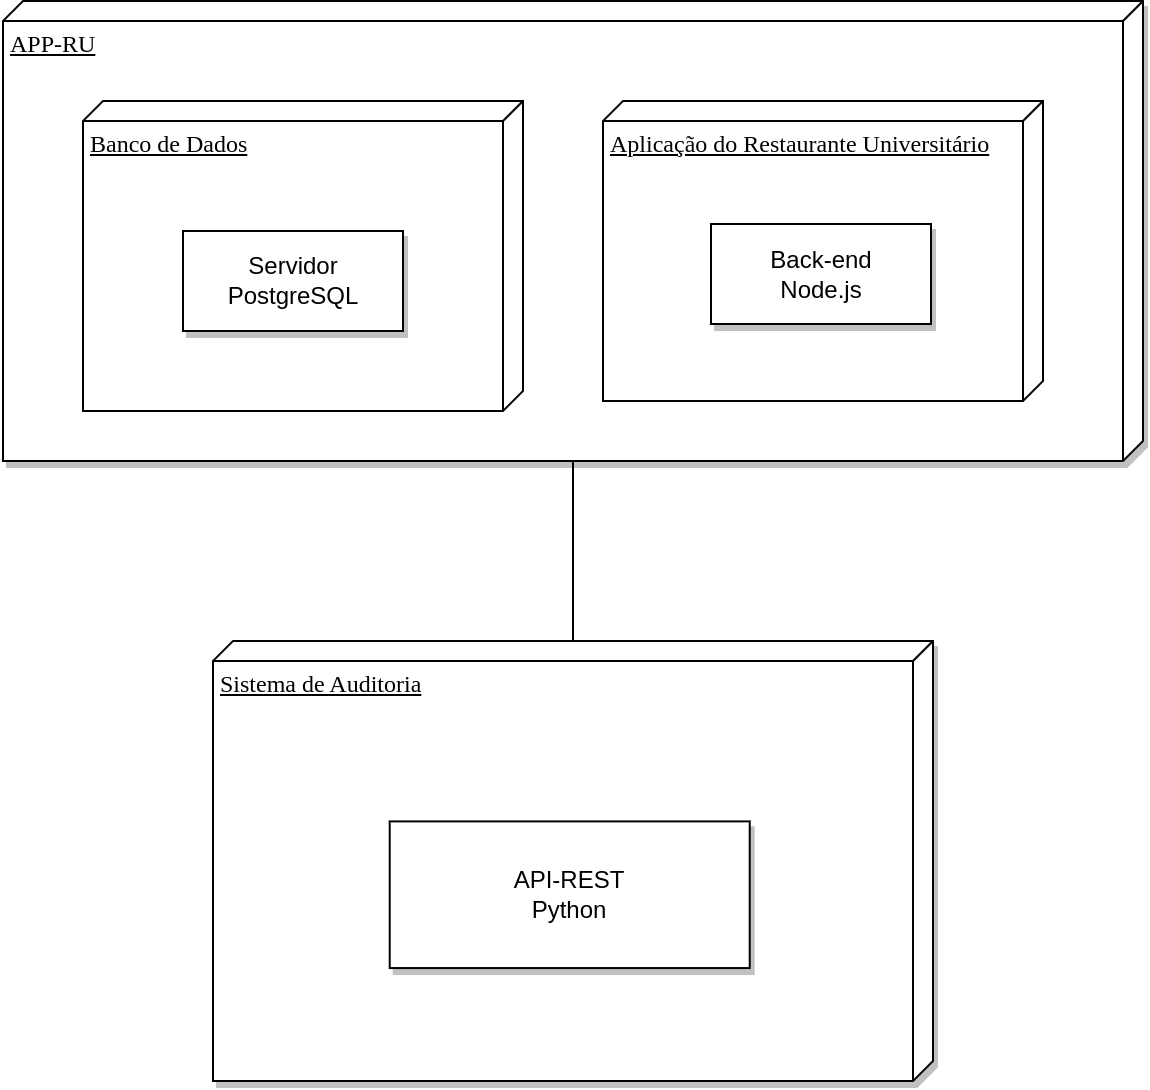
\includegraphics[width=0.8\textwidth]{img/Cap3/diagramas/Diagrama de Implantação.drawio.png}
    \caption{Diagrama de Implantação da aplicação}
    \label{fig:diagrama_implantacao}
\end{figure}
\subsection{Diagrama de Implantação}
O Diagrama de Implantação mostra as necessidades do sistema quanto ao \emph{hardware} a ser utilizado. Em termos práticos, este diagrama elenca os diferentes nós presentes no sistema e suas características, que, segundo \cite{Guedes2018}, são características físicas como servidores, estações, topologias e protocolos de comunicação, ou seja, todo o aparato físico sobre o qual o sistema deverá ser executado.

Componentes de \emph{software} executados, chamados de artefatos, também aparecem no diagrama, como demonstrado na Figura \ref{fig:diagrama_implantacao}. As interações entre os nós a partir de sua conectividade é uma importante informação expressa pelo diagrama de implantação.


\newpage
\subsection{Diagrama de Classes}
\begin{figure}
    \centering
    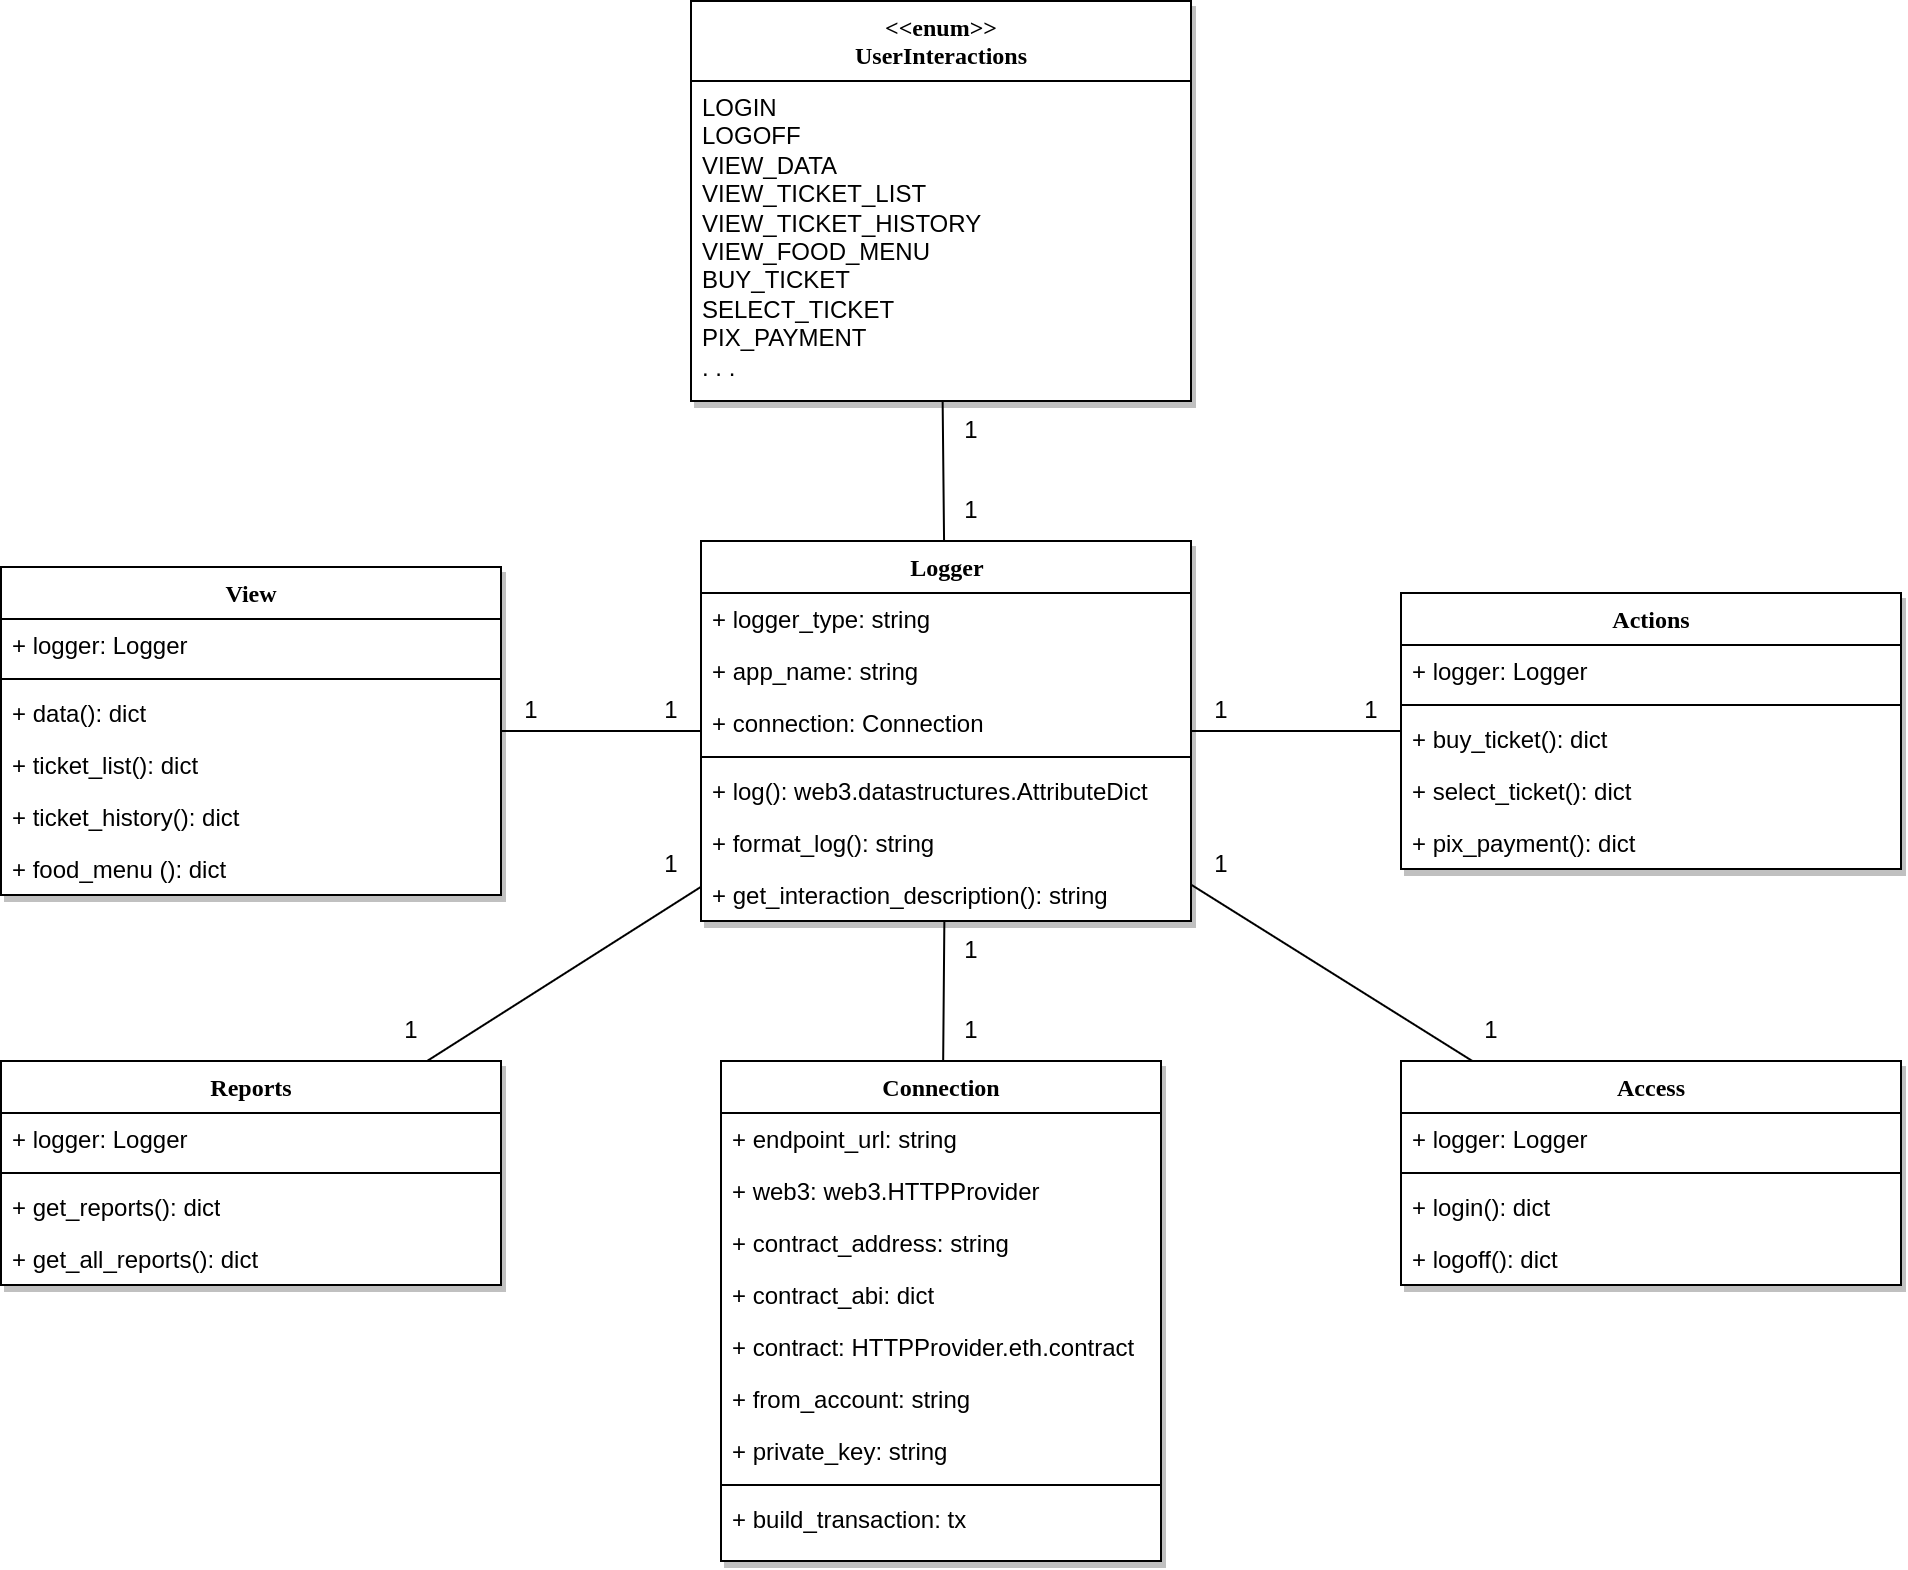
\includegraphics[width=1\textwidth]{img/Cap3/diagramas/Diagrama de Classes.png}
    \caption{Diagrama de Classes da aplicação}
    \label{fig:diagrama_classes}
\end{figure}

Um Diagrama de Classes define as classes presentes no sistema e seus relacionamentos. Uma classe é a base para um objeto que será instanciado e utilizado na aplicação. Cada classe possui atributos e métodos próprios, além da possibilidade de realizar associações entre si.

Quatro das classes retratadas no diagrama da Figura \ref{fig:diagrama_classes} se referem aos diferentes tipos de interações que são interpretadas pela API:
\begin{itemize}
    \item A classe Access implementa métodos de acesso ao sistema, como \emph{login} e \emph{logoff}
    \item A classe Actions implementa métodos de ações gerais realizadas pelo usuário, como a compra de um ticket
    \item A classe View emprega funcionalidades de visualização de dados em geral
    \item A classe Reports dá suporte à obtenção de dados salvos e à geração de relatórios
\end{itemize}

O centro de toda a aplicação jaz na classe Logger. Esta classe tem por objetivo criar as mensagens de \emph{logs} que serão persistidas na rede Blockchain. Para isso, utiliza uma instância da classe Connection, responsável por realizar a conexão com a plataforma Ethereum e realizar operações diversas. A classe Logger também faz uso de uma classe de suporte chamada UserIteractions, enumerando os tipos de interações possíveis dentro do contexto da aplicação.


\section{Implementação da solução}
O sistema de auditoria tem como base uma API REST implementada na linguagem de programação Python, sendo responsável por captar requisições de um cliente e as processar. A depender do tipo de requisição recebida, o sistema apresenta diferentes tipos de comportamentos e estrutura suas respostas de maneira análoga. \emph{Endpoints}, ou pontos de extremidade de uma API, são os locais onde são recebidas as chamadas ao sistema. Estes \emph{endpoints} são chamados por meio de \emph{URIs} específicas, que por sua vez são mapeadas diretamente a funções dentro da aplicação Python.

A API REST, devido à sua conexão com a rede Ethereum, provê dois tipos diferentes de chamadas: funções que alteram o estado e funções que visualizam o estado. Devido à natureza de uma Blockchain, transações realizadas na rede necessitam de um pagamento para serem concretizadas, ao tempo que operações de leitura da rede não possuem custo operacionais. A escrita de mensagens de \emph{log} é um ato de persistência de informação na rede, possuindo assim um certo custo inerente; a visualização destes \emph{logs}, por sua vez, é um ato não dispendioso.

A implementação da API REST deu-se a partir de uma imagem Docker da linguagem de programação Python. Desta forma, todas as dependências da aplicação são isoladas de todo o resto do sistema, reduzindo drasticamente problemas de conflito de versões e aumentando a portabilidade da solução.

\subsection{Conexão com a plataforma Ethereum}
\begin{figure}
    \includegraphics[width=0.4\textwidth]{img/Cap3/blockchain/Conexão 1.png}
    \centering
    \includegraphics[width=0.4\textwidth]{img/Cap3/blockchain/Conexão 2.png}
    \caption{Demonstração da implantação de um contrato inteligente via MetaMask}
    \label{fig:smart_contract}
\end{figure}
Para manipular dados na Blockchain é necessário ter em posse uma carteira de criptomoedas, possibilitando assim a realização de transações na rede. Como existem várias maneiras de se criar uma carteira, optou-se pelo uso do \emph{software} MetaMask para sua criação e manutenção. O MetaMask é uma extensão de navegador que permite que usuários armazenem e gerenciem contas, além de possibilitar a comunicação com aplicações descentralizadas. A Figura \ref{fig:smart_contract} mostra uma carteira configurada com diferentes contas.

A partir da carteira criada pelo MetaMask, criaram-se contas capazes de serem usadas na rede Ethereum e suas \emph{testnets}. Cada conta é composta em sua essência por um par de chaves: a chave pública e a chave privada. A chave pública é derivada da chave privada e pode ser compartilhada e usada por qualquer um para verificar assinaturas digitais feitas pela chave privada, que por sua vez é utilizada para comprovar posse de contas ou contratos da Blockchain. 

\begin{figure}
\centering
    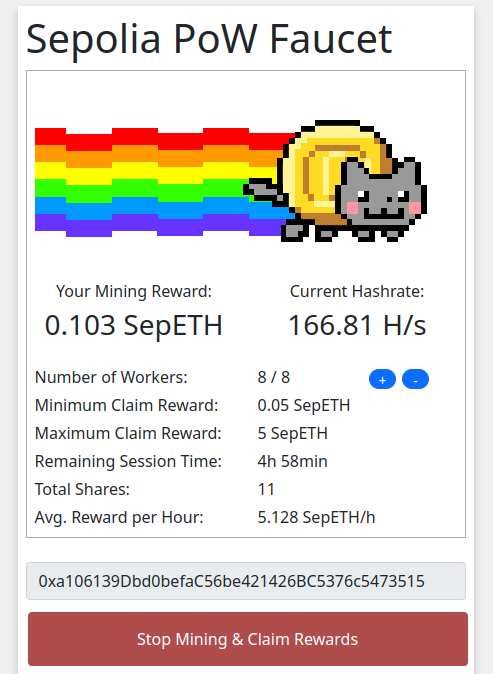
\includegraphics[width=0.5\textwidth]{img/Cap3/blockchain/faucet.png}
    \caption{Obtenção de criptomoedas de teste para a \emph{testnet} Sepolia}
    \label{fig:faucet}
\end{figure}

As quantias de criptomoedas das contas criadas são provenientes de  \emph{faucets}. Cada \emph{faucet} costuma ser especializada em uma \emph{testnet} específica. Particularmente, a principal \emph{faucet} utilizada foi a Sepolia PoW Faucet \cite{pow_faucet}, hospedada em \emph{websites} que se dispõem a depositar Ether à um endereço da Blockchain em troca de tarefas de mineração concretizadas pelo computador do usuário. A quantidade de criptomoeda recebida é proporcional ao tempo e esforço computacional realizado. A Figura \ref{fig:faucet} demonstra um processo de mineração em andamento pelo \emph{website}, provendo uma remuneração com base na quantidade de cálculos executados pelo computador.

Para salvar as mensagens de \emph{log} foi implementado um contrato inteligente na linguagem de programação Solidity; desta forma, é possível executar chamadas ao contrato após o seu processo de implantação na rede (\emph{deploy}). O desenvolvimento do contrato se deu por meio da plataforma Remix IDE, que provê um ambiente de desenvolvimento próprio para a confecção de contratos inteligentes. Após sua escrita, o contrato é compilado para então, finalmente, ser lançado na rede Ethereum. 

O contrato inteligente implementa uma estrutura de dados chamada \emph{mapping}, que mapeia uma determinada entrada a uma única saída, similar a uma tabela de dispersão (também conhecida como \emph{hash}). Devido a natureza da Blockchain, operações de persistência na rede exigem certa quantidade de criptomoeda para serem executadas; para isso, realiza-se a criação de uma transação a partir dos dados recebidos, que é assinada com a chave privada da conta utilizada pela API. Isso garante o envio da transação de forma única e inequívoca por parte do sistema. O dado utilizado na estrutura de mapeamento é o id, a identificação única do usuário no contexto do sistema, que aponta para uma estrutura de dados do tipo lista, responsável por guardar as mensagens de log recebidas pela aplicação. Operações de visualização de dados, por sua vez, não possuem custo de execução e podem ser executadas livremente, retornando para a API REST todos os dados salvos. Como o contrato inteligente é um endereço público na Blockchain, uma camada de segurança, em tempo de execução do contrato, foi empregada: apenas a conta que é dona do contrato, ou seja, a conta que realizou a implantação do contrato na rede, é capaz de chamar os métodos do contrato.

\begin{figure}
    \centering
    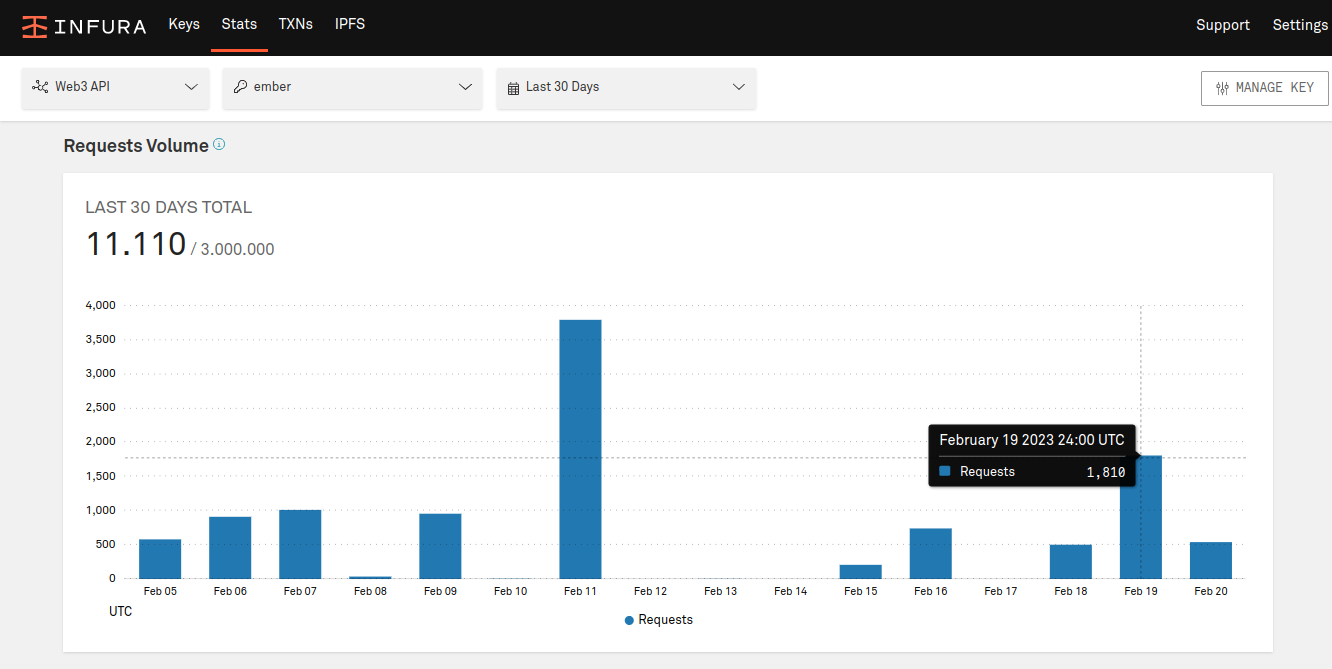
\includegraphics[width=1\textwidth]{img/Cap3/blockchain/Infura estatisticas.png}
    \caption{Gráfico de requisições realizadas fornecido pelo provedor Infura}
    \label{fig:infura_estatisticas}
\end{figure}
Para interagir com o contrato inteligente, a API REST necessita se comunicar com a Blockchain. Esta necessidade é sanada com o uso de um provedor Infura. Infura é o nome de um serviço de estrutura de nó (\emph{node infrastructure}) que provê acesso confiável para a rede Ethereum. A partir de sua API, o Infura permite acesso instantâneo à rede por meio do protocolo HTTPS e de WebSockets. A biblioteca Web3.py faz uso da url do provedor, que contém a chave de API necessária para concretizar a comunicação.

A partir da conexão com o provedor Infura, é possível fazer chamadas ao contrato inteligente implantado na Blockchain. A biblioteca Web3.py é capaz de fazer chamadas a métodos do contrato após a sua implantação na rede com o uso de seu endereço único. Para isso, são passados os parâmetros correspondentes necessários para a chamada de uma função do contrato. A plataforma disponibiliza um \emph{dashboard}, tal como na Figura \ref{fig:infura_estatisticas}, para a visualização de estatísticas de uso do provedor, como o número de requisições efetuadas em determinado período de tempo.

\begin{figure}
\centering
    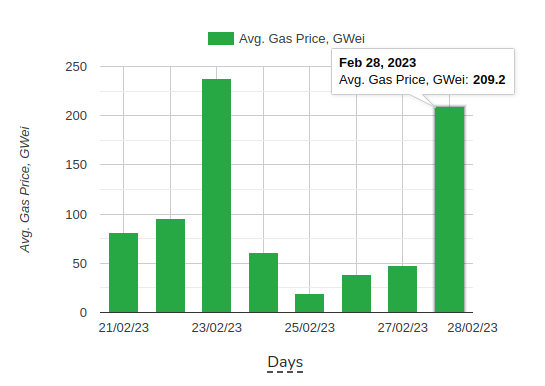
\includegraphics[width=0.8\textwidth]{img/Cap3/blockchain/goerli gas.png}
    \caption{Súbita variação do preço de \emph{gas} na \emph{testnet} Goerli \cite{Bitquery}}
    \label{fig:goerli_gas}
\end{figure}
A escolha da \emph{testnet} utilizada baseou-se na alternativa mais bem difundida, que é a rede Goerli. No entanto, altas flutuações no tráfego da rede a tornaram uma alternativa inviável devido ao súbito aumento do preço do \emph{gas}, como expresso no gráfico da Figura \ref{fig:goerli_gas}. Segundo Marius van der Wijden, desenvolvedor da plataforma Ethereum, este encarecimento no preço das transações da rede é um comportamento esperado com todas as \emph{testnets} \cite{kelly_2023}. Segundo o desenvolvedor, o plano é fazer uma lenta migração de usuários da rede Goerli para a rede Sepolia. A rede Sepolia foi criada com o intuito de ajudar desenvolvedores testarem suas aplicações descentralizadas em um ambiente mais realista e que mais se assemelha à \emph{mainnet} Ethereum \cite{porcelli_2023}. Portanto, optou-se por migrar o contrato inteligente implementado para a \emph{testnet} Sepolia, sem grandes perdas. 


\subsection{Mensagens de \emph{log}}
O sistema de auditoria para o aplicativo Carteira Digital do Restaurante Universitário da UEA tem por objetivo registrar, de forma permanente, as interações realizadas pelos usuários do aplicativo. Atos como entrar no aplicativo, a compra de um ticket de alimentação e a visualização do cardápio são registradas de maneira segura na rede Blockchain, impedindo assim quaisquer ações com o intuito de adulteração de dados. Os registros, ou \emph{logs}, possuem a seguinte estrutura:

\begin{table}[H]
    \centering
    \begin{tabular}{| p{14cm} |}
        \hline
         2023-01-01 08:00:00 APP\_RU:view | 'nome' [id] viewed the food menu \\
        \hline
    \end{tabular}
    \label{tab:estrutura_log}
\end{table}
De forma que cada parte da mensagem possui um significado:
\begin{table}[H]
    \centering
    \begin{tabular}{ | p{4cm} | p{10cm} |}
        \hline
        \textbf{Mensagem} & \textbf{Descrição}\\
        \hline
        
        2023-01-01 & Data da interação a ser registrada, no formato YYYY-MM-DD \\
        \hline

        08:00:00 & Hora da interação a ser registrada, no fuso horário GMT-4 (America/Manaus) \\
        \hline

        APP\_RU:view & Nome da aplicação executada seguida do módulo do sistema \\
        \hline

        | & Caractere delimitador que isola dados da mensagem \\
        \hline

        'nome' {[}id{]} & Nome de usuário no qual ficará registrada a ação efetuada (opcional), dentro de aspas simples; id do usuário, dentro de colchetes \\
        \hline      

        viewed the food menu & Ação efetuada pelo usuário \\
        \hline      
    \end{tabular}
    \caption{Estrutura da mensagem de \emph{log}}
    \label{tab:estrutura_log}
\end{table}

Cada interação configura o registro de um \emph{log} informacional na Blockchain. A estrutura de uma mensagem de \emph{log} é fixa e padronizada com o intuito de facilitar auditorias do sistema, sendo composta por um cabeçalho e um corpo. No cabeçalho são definidos metadados para caracterizar a mensagem de \emph{log} a ser armazenada, sendo utilizadas data, hora e a fonte, referenciando qual parte do sistema foi recebeu uma chamada e foi executada. O corpo da mensagem, por sua vez, carrega consigo a informação necessária para identificar a entidade e sua ação direta no sistema, garantindo assim irretratabilidade ou não repúdio. Desta forma, uma vez executada por um usuário, uma ação não pode ser negada e nem desfeita e sempre apontará para o indivíduo que a realizou.

Para facilitar a visualização, optou-se por separar o cabeçalho e corpo da mensagem por um delimitador, para isso foi utilizado o caractere \emph{pipe} (|), ou barra vertical, com o intuito de alinhar as mensagens em relação ao caractere.

\subsection{Trilhas de auditoria}
\begin{figure}
    \centering
    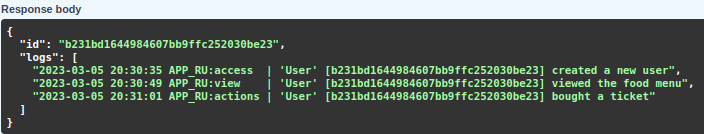
\includegraphics[width=1\textwidth]{img/Cap3/Trilha de auditoria.png}
    \caption{Exemplo de trilha de auditoria fornecida pela API REST}
    \label{fig:trilha_auditoria}
\end{figure}

O conjunto de ações efetuadas pelo usuário, no contexto do sistema, é registrado, compondo assim uma trilha de auditoria acessível a qualquer momento. A trilha de auditoria, sendo um elemento fundamental na responsabilização das partes, deve ser íntegra e corresponder com a realidade, o que é alcançado com o uso da rede Ethereum.

Após o usuário realizar uma ação, uma chamada é disparada à API REST. Num primeiro momento, os dados são capturados e então passam por um processo chamado de serialização, no qual são traduzidos para uma estrutura em que a linguagem de programação consiga entender. Em seguida, as informações são utilizados pela lógica de negócio. 

Para salvar a mensagem correta no \emph{log}, a classe responsável pela sua construção se relaciona com uma classe de suporte chamada UserInteraction, que implementa um Enum, um tipo de dados abstrato utilizado para enumerar um conjunto finito de opções, que neste caso são os tipos de interações possíveis com o sistema. Para cada tipo de Enum presente nesta classe está configurada uma mensagem. A Figura \ref{fig:trilha_auditoria} ilustra diferentes mensagens presentes em uma trilha de auditoria de um usuário.


\section{Integração com o aplicativo Carteira Digital do Restaurante Universitário da UEA}
No processo de desenvolvimento de um sistema, a integração de sistemas é um estágio em que componentes são colocados juntos para a criação de um novo sistema \cite{Sommerville2011}. Para realizar a integração do \emph{back-end} do aplicativo do Restaurante Universitário da UEA, foi necessário, inicialmente, executar o sistema em um ambiente próprio. Com isso, uma análise geral da construção do projeto fez-se necessário, desde a instalação de dependências até um estudo preliminar do código-fonte.

A tecnologia utilizada para o \emph{back-end} da aplicação do RU é o Node.js, um ambiente (\emph{runtime environment}) para servidores orientados a eventos que faz uso da linguagem de programação Javascript para processar requisições de clientes. Junto ao Node.js, o projeto emprega o \emph{software} PostgreSQL para atuar como SGDB (Sistema de Gerenciamento de Banco de Dados) da aplicação, responsável por criar, manter e manipular bancos de dados. Para dar suporte à tarefas de banco de dados, o sistema recorre ao Prisma, um ORM (\emph{Object-Relational Mapper}) ou mapeador objeto-relacional com o intuito de mitigar riscos envolvidos na livre escrita de consultas de dados na aplicação, como ataques de injeção SQL e agilizar o desenvolvimento da aplicação.

\begin{figure}
    \centering
    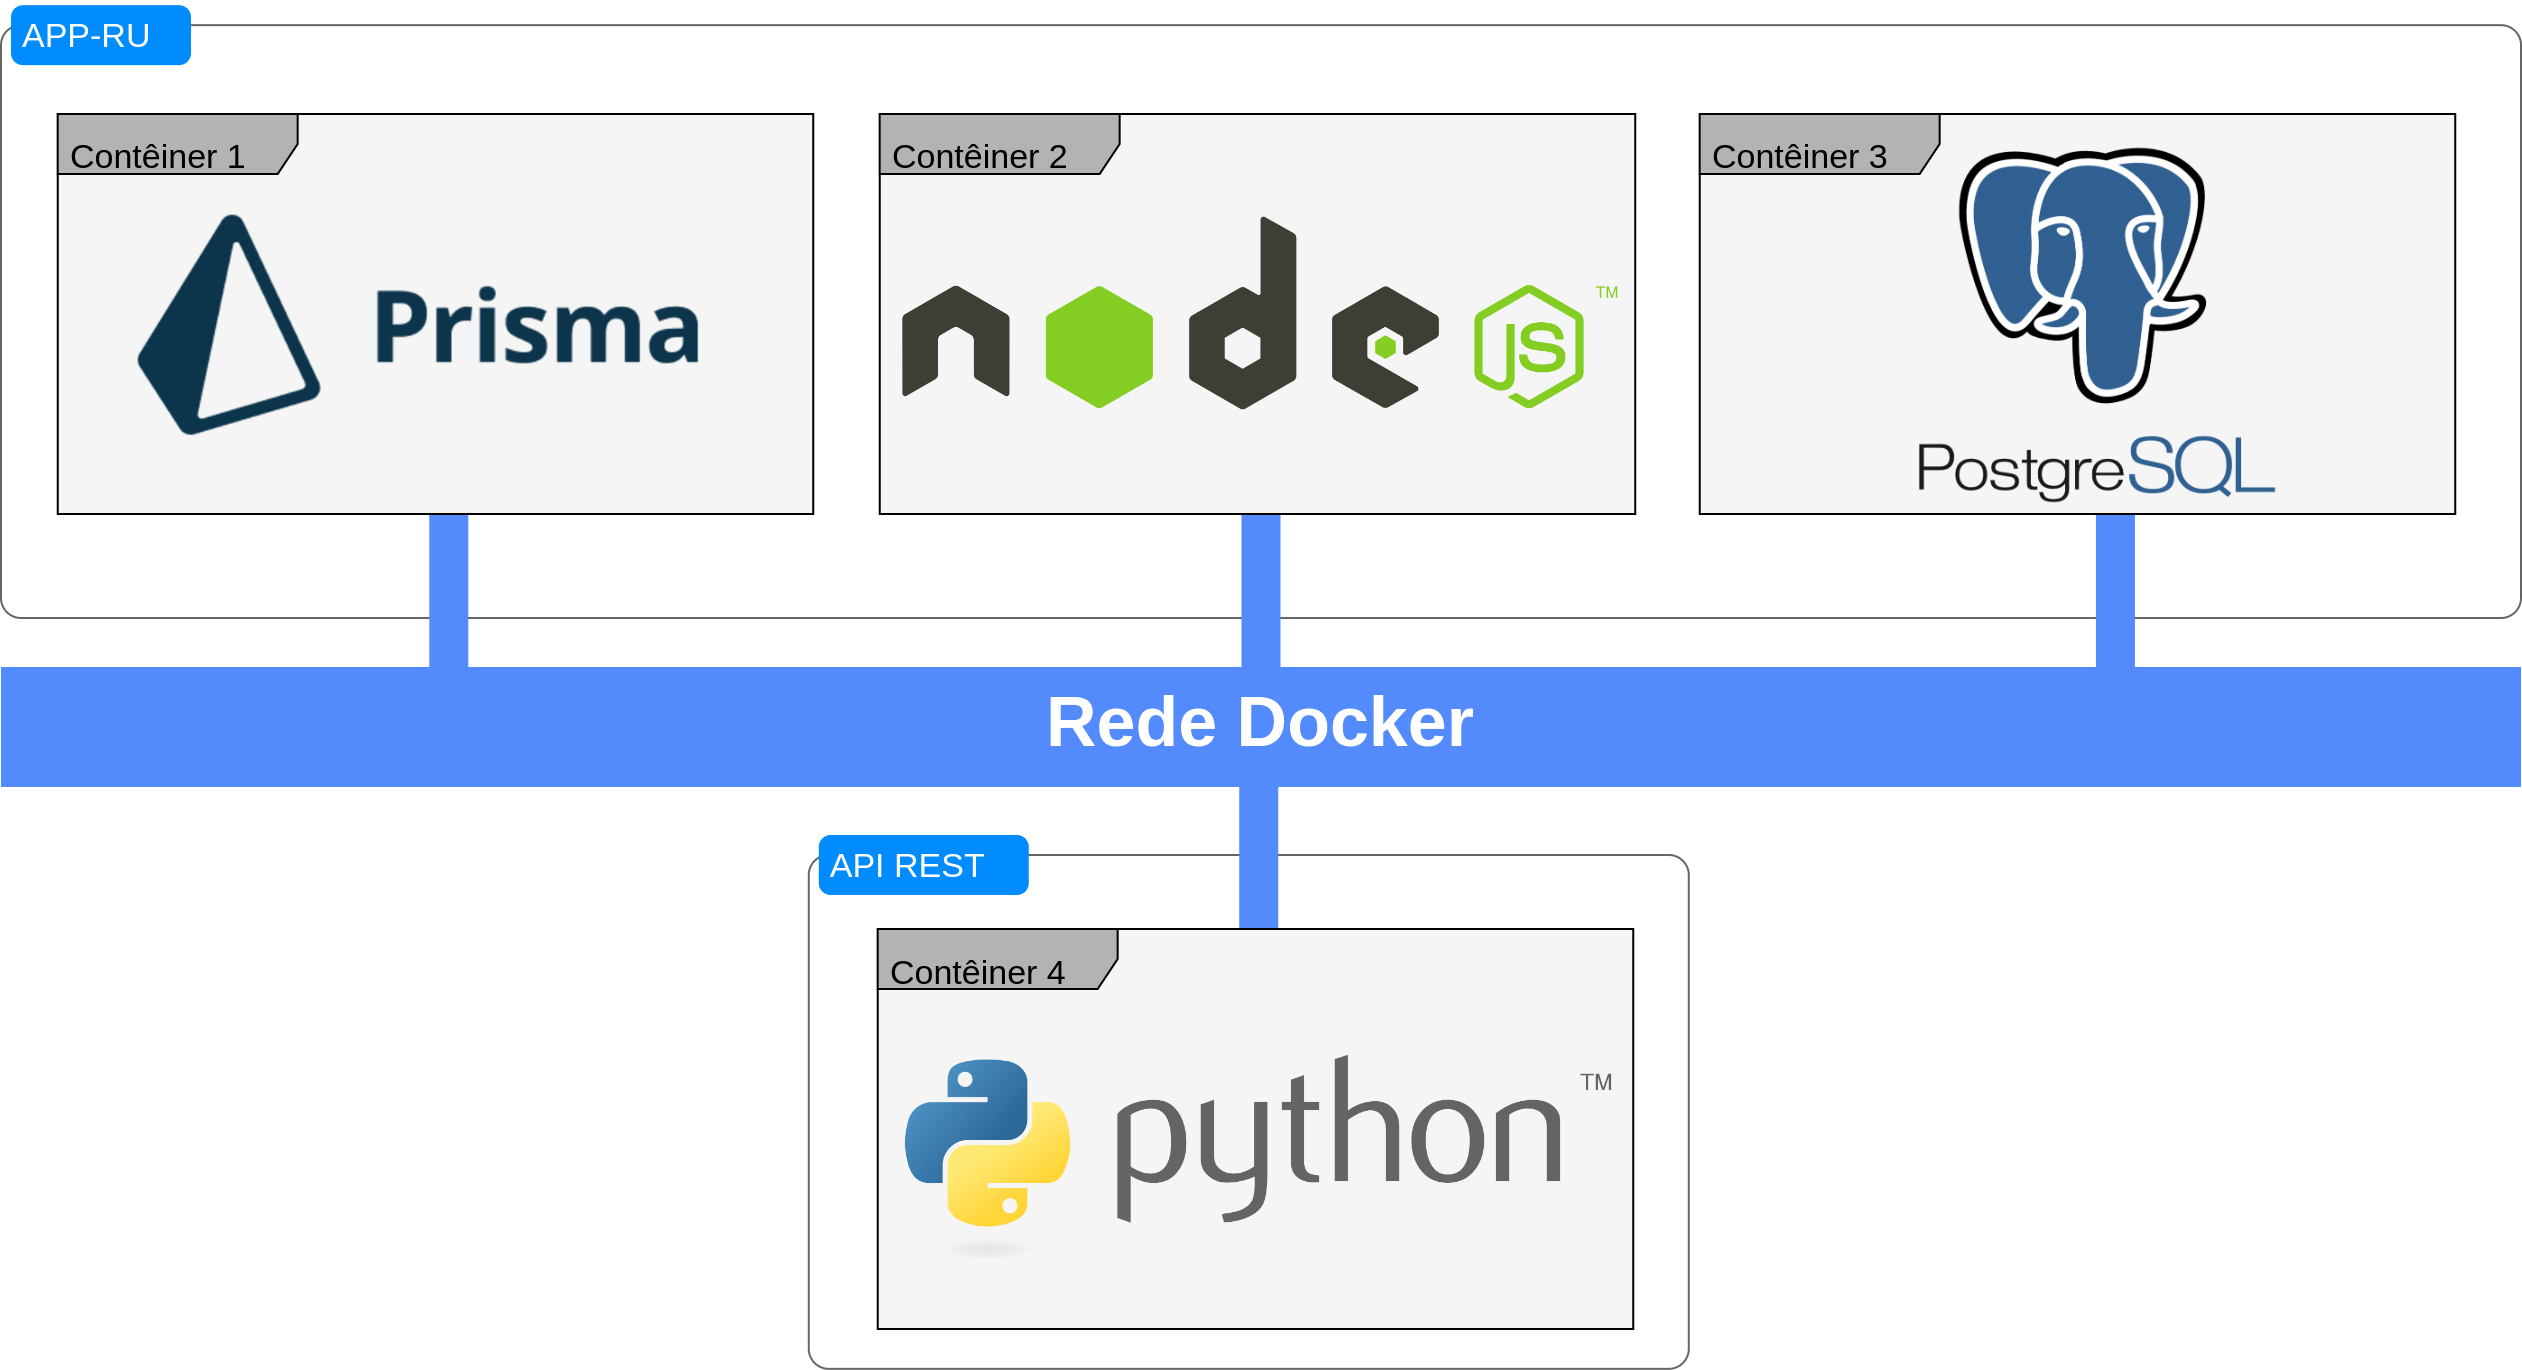
\includegraphics[width=1\textwidth]{img/Cap3/Rede Docker.png}
    \caption{Rede formada pelos diferentes contêineres com o docker-compose}
    \label{fig:rede_docker}
\end{figure}


Todas as tecnologias descritas anteriormente integram-se a partir do Docker, que é responsável por executar um contêiner por serviço e gerenciar as comunicações entre cada um deles. O diagrama da Figura \ref{fig:rede_docker} ilustra a conexão entre os diferentes contêineres. Para isso, utiliza-se a ferramenta \emph{docker-compose}, fazendo com que cada um dos contêineres passem a se enxergar e comuniquem-se entre si de forma totalmente transparente, como em uma rede. O \emph{docker-compose} é uma ferramenta que define os componentes de uma aplicação (como contêineres, volumes e configurações) em um único arquivo \cite{Raj2015-ju}, garantindo assim ao desenvolvedor a possibilidade de executar o sistema mais facilmente, simplificando instalações e futuras implantações do \emph{software}.

Parte do esforço de integração entre diferentes sistemas se dá, num primeiro momento, na configuração do ambiente de ambas as partes a serem integradas. Segundo \cite{Sommerville2011}, em integrações entre diferentes sistemas a fim de se criar um único, uma fração significativa do desenvolvimento preocupa-se com a configuração do sistema e não com o desenvolvimento de código original. 

Adaptações necessárias ao código fonte do APP-RU também foram necessárias, a fim de que passe a ser registrada cada ação tomada por um usuário deste sistema. No caso de um utilizador do sistema criar um novo usuário para si, visualizar o cardápio do restaurante e em seguida comprar um ticket, cada uma destas ações é registrada de forma individual, garantindo rastreabilidade nos passos seguidos por este utilizador da aplicação. Para isso, incluiu-se no código-fonte chamadas à API REST, conforme o tipo de requisição processada pelo \emph{back-end} do APP-RU.


\section{Testes na aplicação}
Testes de \emph{software} foram implementados para garantir qualidade à aplicação desenvolvida, além de promover a redução de risco de falhas, devido à descoberta de possíveis erros de execução. A abordagem escolhida foi a utilização de testes de caixa-preta para testar os \emph{endpoints} da API REST. Os tipos de testes empregados são testes de unidade e testes de integração.

Os testes de unidade são utilizados para testar unidades individuais para o sistema, que para \cite{Pressman2021-jj} são os componentes, com a finalidade de garantir que sua função esteja sendo desempenhada de maneira correta. Testes de integração, por sua vez, visam testar a conjunção de diferentes componentes que interagem entre si \cite{Pressman2021-jj}. É um tipo de teste necessário pois mesmo que dois componentes distintos funcionem normalmente de forma isolada, existe a chance de que haja algum tipo de erro na ponte que faz ligação com ambos, ou seja, na interface.

Após ser realizada uma transação na Blockchain, a rede retorna um objeto contendo metadados desta transação, que são utilizados como parâmetro principal do teste realizado. Um atributo deste objeto é o atributo \emph{status}, que pode possuir ou o valor 1, denotando sucesso na transação, ou o valor 0, denotando uma falha no processo. Esta resposta recebida pela Blockchain após ser realizada uma transação é o que fundamenta o teste. Erros em tempo de execução também são levados em conta: se houver qualquer tipo de exceção não tratada dentro do código, o teste falha, apontando o erro e a linha onde ele ocorreu.

\subsection{Testes de unidade e integração}
\begin{figure}
    \centering
    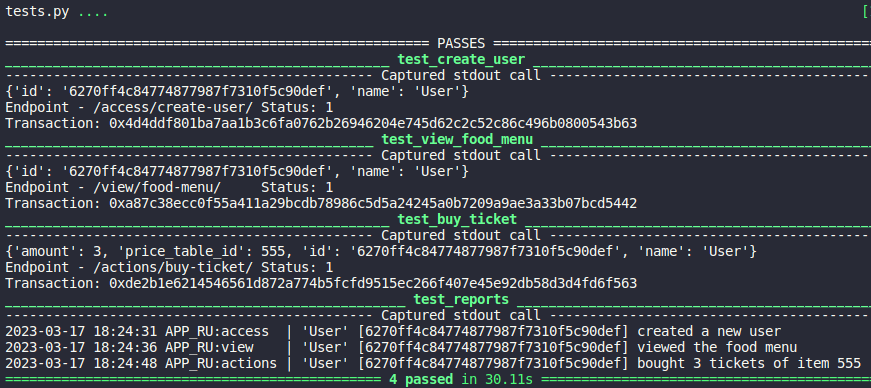
\includegraphics[width=1\textwidth]{img/Cap3/teste de unidade.png}
    \caption{Teste de unidade realizado com id gerado de forma aleatória}
    \label{fig:teste_unidade}
\end{figure}

Para realizar os testes de unidade e de integração foi utilizada a ferramenta pytest. Ela executa um código composto por diversas funções prefixadas com a palavra "\emph{test}", cada uma referenciando um caso de teste diferente, observando a aparição de possíveis erros no código em tempo de execução. Caso não haja nenhum tipo de erro, é dito que a função executada foi bem sucedida e passou no teste.

Devido à grande quantidade de \emph{endpoints} diferentes, optou-se por testar um \emph{endpoint} para cada módulo do sistema devido ao fato de cada módulo implementar uma classe única. Desta forma, foram escolhidos os \emph{endpoints} de criação de usuário, de visualização do cardápio e de compra de ticket.

A biblioteca pytest executa funções encarregadas de mandar requisições para a API REST. A depender do \emph{endpoint}, diferentes argumentos são passados para concretizar a requisição e estruturar a mensagem de \emph{log}. Os testes de unidade são realizados por meio de chamadas diretas à API REST, visando testar o funcionamento dos módulos. Os testes de integração, por sua vez, são feitos com chamadas à API REST realizadas pelo \emph{back-end} da aplicação do Restaurante Universitário. Ambos os testes possuem a mesma saída, que é expressa na Figura \ref{fig:teste_unidade}.


